\documentclass[a4paper]{scrreprt}
\usepackage{fancyhdr}
\pagestyle{fancy}
\usepackage[english]{babel}
\usepackage[utf8]{inputenc}
\usepackage{graphicx}
\usepackage{url}
\usepackage{textcomp}
\usepackage{amsmath}
\usepackage{lastpage}
\usepackage{pgf}
\usepackage{wrapfig}
\usepackage{fancyvrb}
\usepackage{appendix}
\usepackage{pdfpages}
\usepackage{xcolor}
\usepackage{hyperref}

\hypersetup{
    colorlinks=true,
    linkcolor=blue,
    filecolor=black,      
    urlcolor=blue,
    citecolor=black,
}

% Create header and footer
\headheight 27pt
\pagestyle{fancyplain}
\lhead{\footnotesize{Datalagring, IV1351}}
\chead{\footnotesize{Task 2}}
\rhead{}
\lfoot{}
\cfoot{\thepage\ (\pageref{LastPage})}
\rfoot{}

% Create title page
\title{Task 2}
\subtitle{Datalagring, IV1351}
\author{Adrian Jonsson Sjödin \\ adriansj@kth.se}
\date{\today} 


\begin{document}

\maketitle

\tableofcontents %Generates the TOC

\chapter{Introduction}
The purpose of task 2 was to turn the conceptual model of the Sound Good Music School database developed in task 1, into a logical model. That is a model that we can 
use when creating our database in MySQL. The creation and reasoning behind this logical model is what will be covered in this report.

\chapter{Method}
To turn our conceptual model (see fig. \ref{fig:conceptualModel}) into a logical model we mostly followed the steps laid out in the lecture about logical and physical models.

First we copied our conceptual model into the logical model and then proceeded to delete all relationships so that we where only left with the tables, and after this we 
went through each table and made sure they where 1NF and no row contained duplicated. This resulted in some new tables. After this we specified the type for each column 
and whether or not it should allow NULL.

Then the next step was to achieve 2NF and start creating the Primary Keys and draw the relationships between the tables, and consider which Foreign Keys can be allowed 
to be NULL. Drawing the relationships resulted in some tables being deleted.

The last step was to split up some tables a bit more to try and achieve 3NF.

Having the logical model done we created the database using Astah's export to SQL function. Unfortunately you can not directly use it since it gave quite a lot of errors,
but it gave a good foundation to build upon.

For writing the SQl scripts that created the databases and populated it with data MySQL Workbench and DBGate was used. The logical model was created in Astah. 





\begin{figure}[h]
    \begin{center}
        \includegraphics[width=\textwidth]{../img/conceptualModel.v1.0.1.png}
        \caption{Conceptual Model for the SoundGood music school database}
        \label{fig:conceptualModel}
    \end{center}
\end{figure}


\chapter{Result}
\label{sec:result}
In figure \ref{fig:logicalModel} we can see the finished Logical Model. The SQL scripts can be found here:
 \href{https://github.com/adrian-jonsson-sjoedin/IV1351-Datalagring/tree/main/project/SQL}{GitHub}.


\begin{figure}[h]
    \begin{center}
        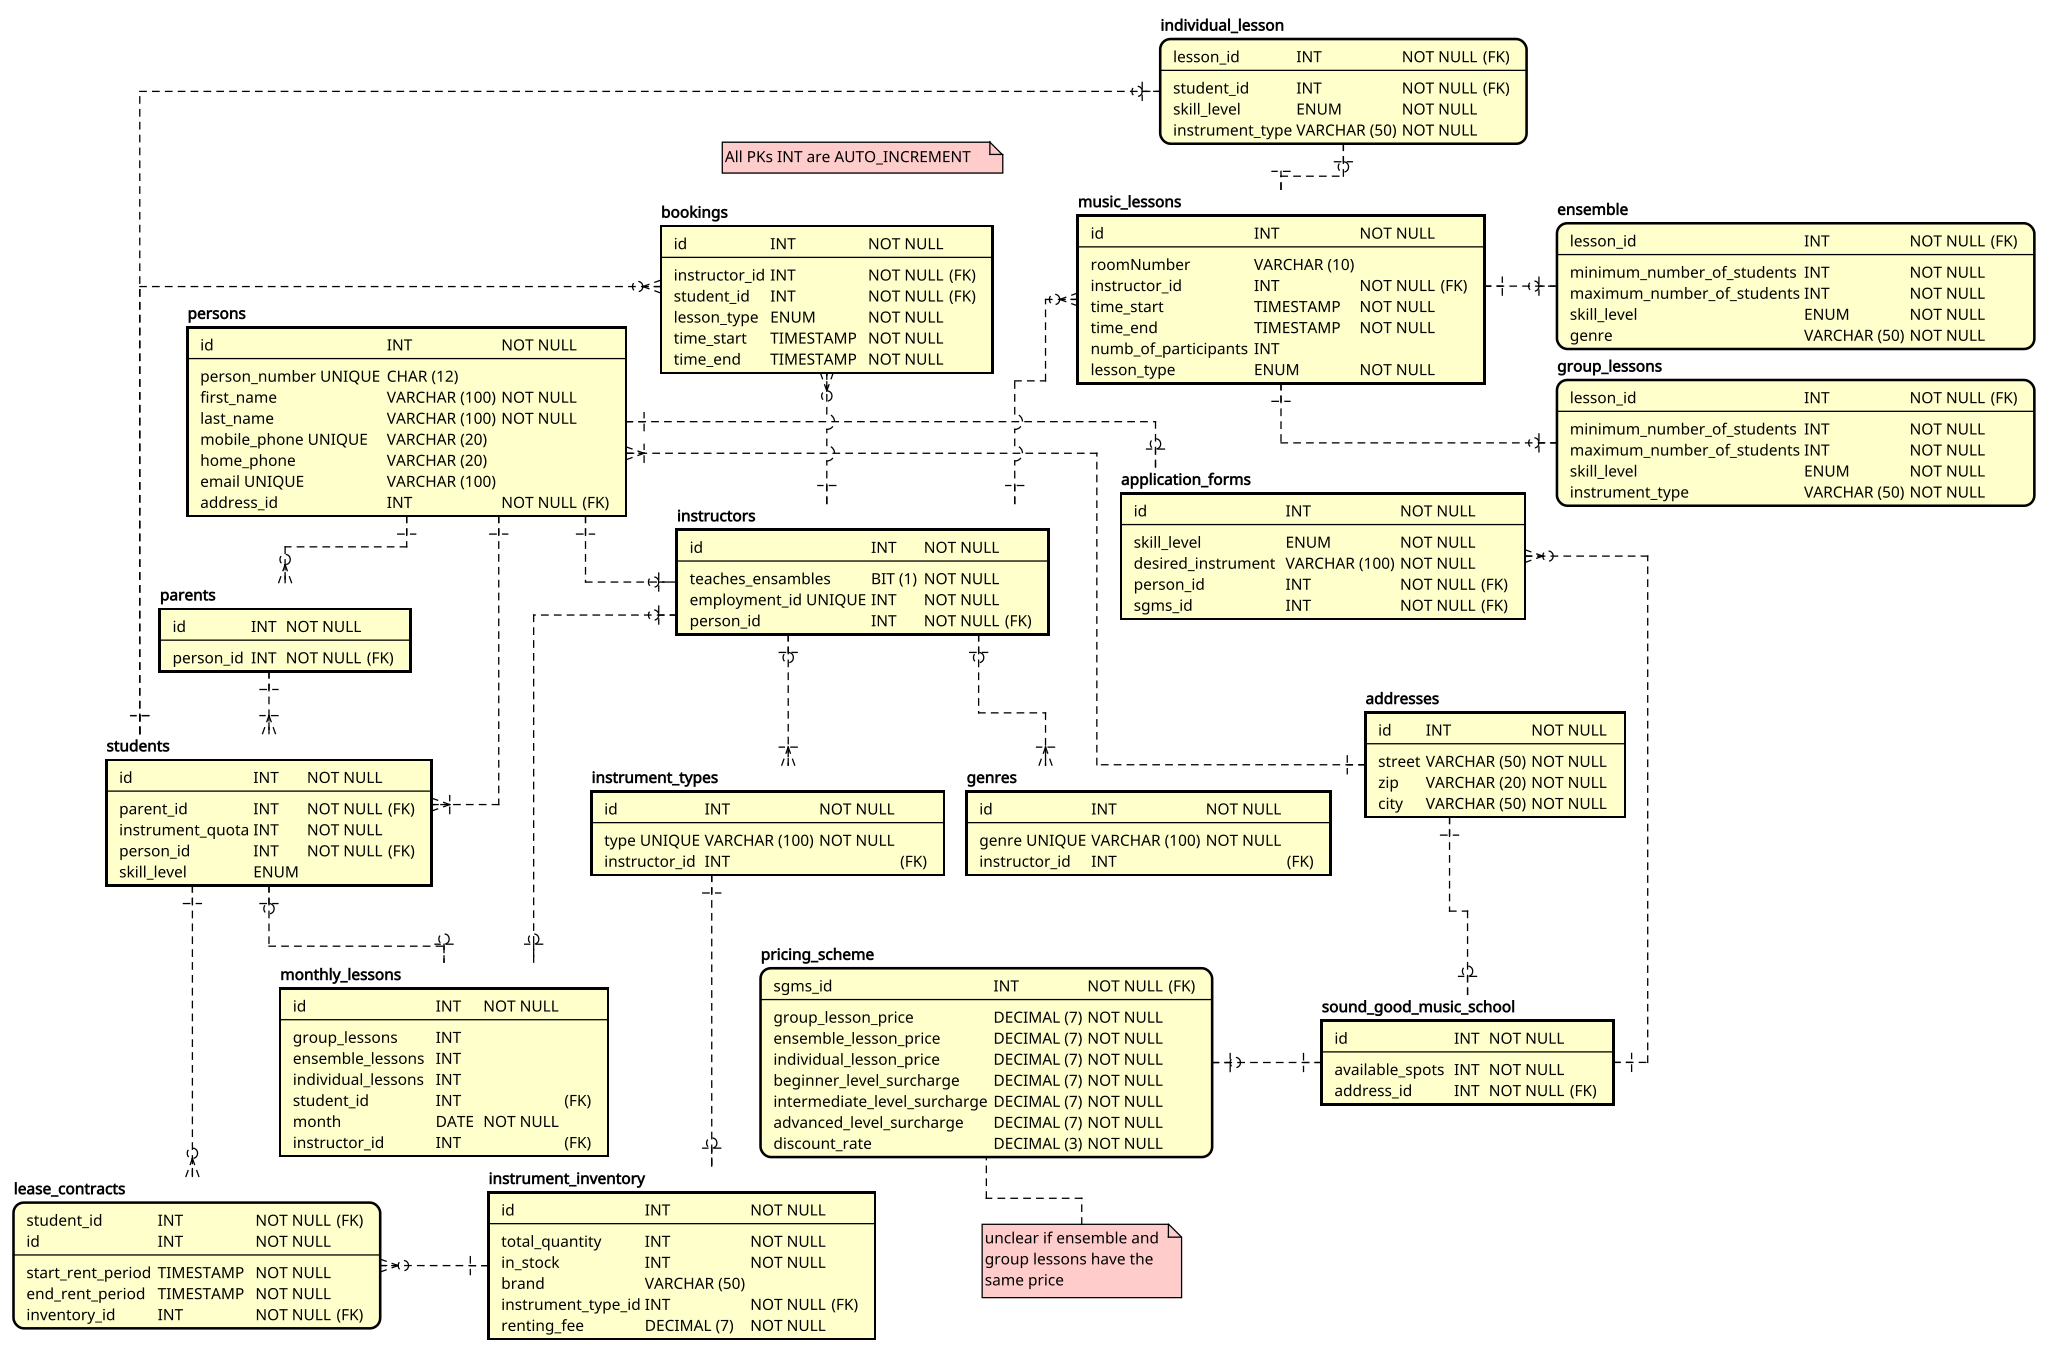
\includegraphics[width=\textwidth]{../img/LogicalModel.png}
        \caption{Logical Model for the SoundGood music school database}
        \label{fig:logicalModel}
    \end{center}
\end{figure}

I tried to have as little duplicated data as possible which is why I decided to have a table "addresses" instead of combining it with both "persons" and 
"sound\_good\_music\_school". They will instead have a Foreign Key to the address, which will keep the table smaller and save memory since we will not have multiple
rows with the same values for people living at the same address. The same reasoning is behind the "parents" and "students" table with them having a Foreign Key to 
"persons".

We also have zero derived data in the tables with the one exception being "monthly\_lessons". The reason for this will be addressed in the Discussion section.


\chapter{Discussion}
While converting the Conceptual Model into a Logical Model I noticed quite a few flaws that needed correcting. For starters I had the administrative staff in the database,
which is not a requirement since their roll was to use an application that interacts with the database. They handle the bookings and such but the task here was not to 
model a booking system but rather a database system. 

I also added a table "parents" since I realized having an attribute "hasContactPerson" is not the best way to store data about a students parents. Instead "student" now 
have a Foreign Key referencing "parents" and "parents" have a Foreign Key referencing "person". This will also help us calculate which students are siblings since they 
will have the same Foreign Key to parents. 

Another big change is how instruments and the leasing of them is handled. I moved the "instrumentQuota" into "students" and "instrumentFee" into "instrument\_inventory"
thus removing the "InstrumentLease" table seen in fig. \ref{fig:conceptualModel}. The "instrumentLeaseContract" then became the "lease\_contract" and since the same 
student can rent multiple instrument we hade the make the Primary Key a Composite Key using the Foreign Key from "students" and a Surrogate Key. So each row in this
table would represent a lease contract. For the instruments I decided against assigning each single instrument its own serial number and instead went with the approach
of just storing how many instrument of a certain type we have. This is of course something that would have to be discussed with the client, but doing it this way 
simplified the design. 

Speaking of the instrument type, we also created a new table just for that since it helped reducing the duplication of data in the "instructors" table, and we can use 
it in our "instrument\_inventory" table. The reduction of duplicate data is also the reasoning behind the "genres" table.

In fig. \ref{fig:conceptualModel} we can see that we had two tables named "BookingOfMusicLesson" and "Availability", these have been removed and the tables "bookings"
and "music\_lessons" have been created instead. The "bookings" table is quite straightforward, it contains what lesson have been booked, the id for the student taking it
and the id for the instructor holding it, and the time slot. This is filled in and then matched with a lesson in "music\_lesson" by the external booking application (mentioned in the
task description). The "music\_lesson" table is also thought to be populated by an external system and is the table that contains all the lessons offered by the school.
If the number of participants is NULL in one of the rows that means that nobody has booked a spot in that lesson yet. That attribute is also used when checking if a
class is fully booked or if a class will be canceled because of a lack of participants.

Lastly we have the table mentioned in the Result section that contains derived data, namely the "monthly\_lessons" table. When I first made that table I did not think it 
was derived data. The thought was that each row would contain either the Foreign Key for the instructor or the student and then how many lessons they had taken (or held)
during the month. This in combination with the "pricing\_scheme" table would allow us to calculate the invoice sent to the student or the salary to the instructor. 
However while writing the SQL for creating the database I realized that for the instructors you can get this data from the "music\_lessons" table, and for the students
you can get it by looking at their bookings in combination with the "music\_lessons" table. The bookings have the type of lesson, the instructors id and the time slot, 
which is enough to find the lesson in "music\_lessons", and there we can see if the class was canceled or not. Thus getting how many monthly lessons a student have taken.

I left the table in the Logical Model though because even though it is data that can be derived, it is most likely data we want to store. 

One final thing about the choice of data types and constraints. I used MySQL which is why I went for \textit{CHAR} in the once case where I knew exactly how long a 
string should be. I also used \textit{DECIMAL} since it makes it possible to define exactly how many decimals are allowed. For the constraints only NOT NULL and UNIQUE
are indicated in fig. \ref{fig:logicalModel}, but all \textit{INT}s and \textit{DECIMAL}s have the constraint that they have to be larger or equal to zero.


% This is my first attempt at modeling a database but I think I've gotten everything that was specified in the customer description.
% I have quite a few attributes that are not allowed to be nulled and for those I've simply decided that upon what I think the
% customer would want since it wasn't specified if null values where allowed. For example in the entity \textit{Instructor}
% all three attributes are not allowed to be null, this because it stands to reason that an employer would want to know which
% instruments an instructor knows and what genres they can teach.

% The customer description mentioned that there should be possible to store a contact person for a student, but not that they
% must have one. Because of this I had an entity called \textit{ContactPerson} in an earlier version of my conceptual model, however]
% since I strived to have no duplicated data I had to remove it since that entity then became empty. Instead we have an attribute
% \textit{hasContactPerson} in \textit{Student} that will have a reference to \textit{Person} for the contact person. This is also
% the reason why the attribute \textit{personNumber} can be null, since there is no point in storing the person number for a
% contact person.

% There is also an entity \textit{BookingOfMusicLesson} for which it can be argued that its associations might be a bit weird.
% My thought behind it was that the administrative staff handles a booking by checking what the student wants and then look at
% what is available and can offered to the student. That then books one out of the three lesson types. But reading the name now,
% for example "\textit{BookingOfMusicLesson books IndividualLesson}" does come across a bit strange. Perhaps a better name might
% have been just \textit{MusicLesson}.

% Apart from the above mentioned I believe the conceptual model is sufficient and that it follows the rules and constraints that
% a conceptual model should have. Naming conventions have been followed and every entity has an associations and every attribute
% have its cardinality specified.

\end{document}
